%
% $Id: chapter3.tex 3915 2009-06-18 13:28:32Z sliske $
%
%%\pagestyle{scrheadings}
%%\ohead[]{}
%%\ihead[]{}
%%\chead[]{}
%%\ofoot[\pagemark]{\pagemark}
%%\ifoot[]{}
\chapter{Design \& Implementation}
\label{sec:design}

The following section introduces the design and implementation of the proposed \ac{IPC} architecture and the proof of concept \ac{IPS}, as well as auxiliary libraries and applications.
First, the requirements and the overall purpose of the design are defined and translated into an abstract architecture. Subsequently,  

\section{Requirements}

\section{Abstract Architecture}

\begin{figure}[p]
    \caption[IPC Architecture]{Abstract \ac{IPC} architecture }
    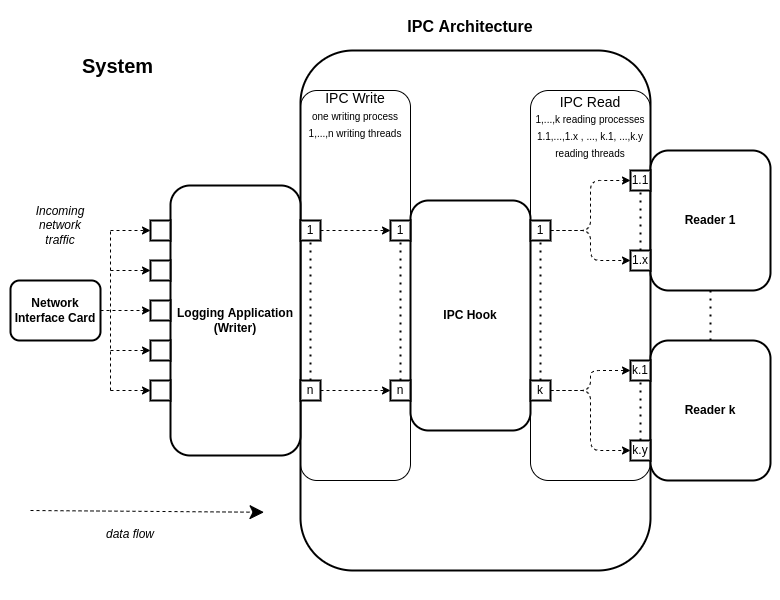
\includegraphics[width=\textwidth]{images/meta_ipc_architecture.png}
\end{figure}

\section{Choice of IPC Type}

\section{Ringbuffer API}

\begin{algorithm}[h!]
    \lstinputlisting[language=c, firstline=27, lastline=36]{listings/shm_ringbuf.h}
    \label{alg:shm:writer_arg}
    \caption[Shared Memory Ringbuffer: Writer Parameters]{this is some text}
\end{algorithm}

\begin{algorithm}[h!]
    \lstinputlisting[language=c, firstline=86, lastline=92]{listings/shm_ringbuf.h}
    \label{alg:shm:set_clean}
    \caption[Shared Memory Ringbuffer: Setup and Cleanup]{this is some text}
\end{algorithm}

\begin{algorithm}[h!]
    \lstinputlisting[language=c, firstline=94, lastline=103]{listings/shm_ringbuf.h}
    \label{alg:shm:write_api}
    \caption[Shared Memory Ringbuffer: Write API]{this is some text}
\end{algorithm}

\begin{algorithm}[h!]
    \lstinputlisting[language=c, firstline=105, lastline=133]{listings/shm_ringbuf.h}
    \label{alg:shm:read_api}
    \caption[Shared Memory Ringbuffer: Read API]{this is some text}
\end{algorithm}

\begin{algorithm}[h!]
    \lstinputlisting[language=c, firstline=39, lastline=46]{listings/shm_ringbuf.h}
    \label{alg:shm:reader_arg}
    \caption[Shared Memory Ringbuffer: Reader Parameters]{this is some text}
\end{algorithm}

\begin{algorithm}[h!]
    \lstinputlisting[language=c, firstline=50, lastline=58]{listings/shm_ringbuf.h}
    \label{alg:shm:global_hdr}
    \caption[Shared Memory Ringbuffer: Global Header]{this is some text}
\end{algorithm}

\begin{algorithm}[h!]
    \lstinputlisting[language=c, firstline=60, lastline=65]{listings/shm_ringbuf.h}
    \label{alg:shm:seg_read}
    \caption[Shared Memory Ringbuffer: Segment Header Reader]{this is some text}
\end{algorithm}

\begin{algorithm}[h!]
    \lstinputlisting[language=c, firstline=67, lastline=71]{listings/shm_ringbuf.h}
    \label{alg:shm_seg_write}
    \caption[Shared Memory Ringbuffer: Segment Header Writer]{this is some text}
\end{algorithm}

\begin{figure}[p]
    \includegraphics[width=\textwidth]{images/shm_architecture.png}
    \caption[Shared Memory Architecture]{Architecture for the single-writer multi-reader shared memory ringbuffer for the transmission
    of log messages. }
\end{figure}

\section{Proof-of-Concept IPS}

\begin{algorithm}[h!]
    \lstinputlisting[language=c, firstline=27, lastline=35]{listings/uring_getline.h}
    \label{alg:uring_getline}
    \caption[io\_uring Getline]{this is some text}
\end{algorithm}

\begin{figure}[p]
    \includegraphics[width=\textwidth]{images/ips_architecture.png}
    \caption[Simplefail2ban Architecture]{Activity diagram for the proof-of-concept IPS implementation. A variable number of ``banning threads'' receive log messages from a host and
    parse them with a predefined regular expressions. For messages that match the expression, the clients IP address is extracted from the log message and added to a hashtable, that keeps count of
    the number of matches per address. If the count reaches the configured limit, the address is added to the list of banned addresses with a current timestamp and inserted into the eBPF map. One ``unbanning
   thread'' routinely iterates through the banned list and checks, if a clients bantime hast elapsed. Clients with an elapsed bantime are removed from the eBPF map, banned list and hashtable.}
   \label{fig:meta_architecture}
\end{figure}

\begin{algorithm}[h!]
    \lstinputlisting[language=c, firstline=29, lastline=38]{listings/ip_hashtable.h}
    \label{alg:ip_hashtable}
    \caption[IP Hashtable]{this is some text}
\end{algorithm}

\begin{table}[h!]
    \label{tab:hash_col}
    \centering
    \small
    \begin{tabular}{llll}
        \toprule
        \textbf{Number of Insertions} & \textbf{Collisions IPv4 [\%]} & \textbf{Collisions IPv6 [\%]} & \textbf{Collisions IPv4 \& IPv6 [\%]}\\ \midrule 
        65534 & 5.33 & 5.29 & 5.28 \\ \midrule
        131068 & 10.17 & 10.17 & 10.15 \\ \midrule
        600011 & 36.81 & 36.77 & 36.8 \\
        \bottomrule
    \end{tabular}
    \caption[Hash Collisions]{Some text}
\end{table}

\section{Test Application}

\begin{table}[h!]
    \label{tab:ip_str}
    \centering
    \small
    \begin{tabular}{lll}
        \toprule
        \textbf{Function} & \textbf{Execution Time IPv4 [Seconds]} & \textbf{Execution Time IPv6 [Seconds]} \\ \midrule 
        inet\_ntop & 1.29 & 3.98 \\ \midrule
        ip\_to\_str & 0.21 & 0.53 \\ 
        \bottomrule
    \end{tabular}
    \caption[IP String Conversion]{Some text}
\end{table}






